\documentclass[prd,aps,twocolumn,a4paper,showkeys,nofootinbib]{revtex4-2}

\usepackage{amsmath}
\usepackage{amsfonts}
\usepackage{amssymb}	
\usepackage{graphicx}
\usepackage{color}
\usepackage[hidelinks]{hyperref}
\allowdisplaybreaks

\def\TODO{\textcolor{red}{TODO:}}
\def\Mc{{\cal M}_c}

\begin{document}

\title{Classification using a random forest}

\author{Marina Berbel}

\date{\today}

\maketitle

%==========================================================
\section{Introduction}
%==========================================================
Working notes on the classification part with a random forest (RF) from scikit-learn. More options could be explored but since now, this tool provides flexibility enough for the task.

The task is to classify events: if they have a neutron star or not, and if they are electromagnetically bright. For now we assume that we work with the dataset from GstLAL early warning, so we only have neutron stars. The goal then is to say if they are bright or not. The label is generated within the dataset by means of the remnant  mass of the merge, for a given equation of state.



%==========================================================
\section{The first try}
%==========================================================
At this time we have two different datasets coming from regression, that we label \textbf{reg1} and \textbf{reg2}.

The dataset \textbf{reg1} contains just the two masses, and not the chirp mass. The regression is done with these two features, and so the output is also these two. It comes from the latest NN from Simone. And the dataset \textbf{reg2} also considers the chirp mass at some point, although the prediction is only the two masses. This comes from Yanyan's NN at IPAM.

So at first we try to use them both with the default random forest, which has as hyperparameters: numer of trees = 100, number of features to use = sqrt(features) = 1 and gini criterion for the information after each split. The rest of the parameters are also the default ones, but we do not mention them because we are not touching them. Also notice that we always let the tree grow as deep as it considers appropriate. Previous tests say that this is the best option.

\subsection{Dependance on initial state}
But we notice that the score of the prediction change every time: the training is dependent on the initial state. We can fix it, but first let's see if the variation is very big. In figure \ref{fig:reg_mean} we can see the mean of the score when we train several times, using injected data, recovered by gstlal and from the NN. The conclusion is that we can have sometimes very good or bad luck with respect to the score from a particular initial condition. But in the long run, we observe that the mean tends to a number, so in average we should get that score whatever the initial condition. This says that we can fix the initial condition for the RF.

Then we can compare the mean score after 2000 trainings, that should be the stable value for the RF with that set of data, when we use the injected data, the values from gstlal and the predicted value with the NN. Also we show as error bars the standard deviation of the score. The results, in figure \ref{fig:compareFirstTry} show that the score is nearly perfect with the injected data. From the other two, it is very similar, so we plot it separately. For \textbf{reg1} they are the same, but for \textbf{reg2} it works better with the data from gstlal.

Anyway none of these scores is above 0.9 and then we cannot call them good. So next step is to fine tune the parameters of the forest for improvement.
\begin{figure*}[]
\center
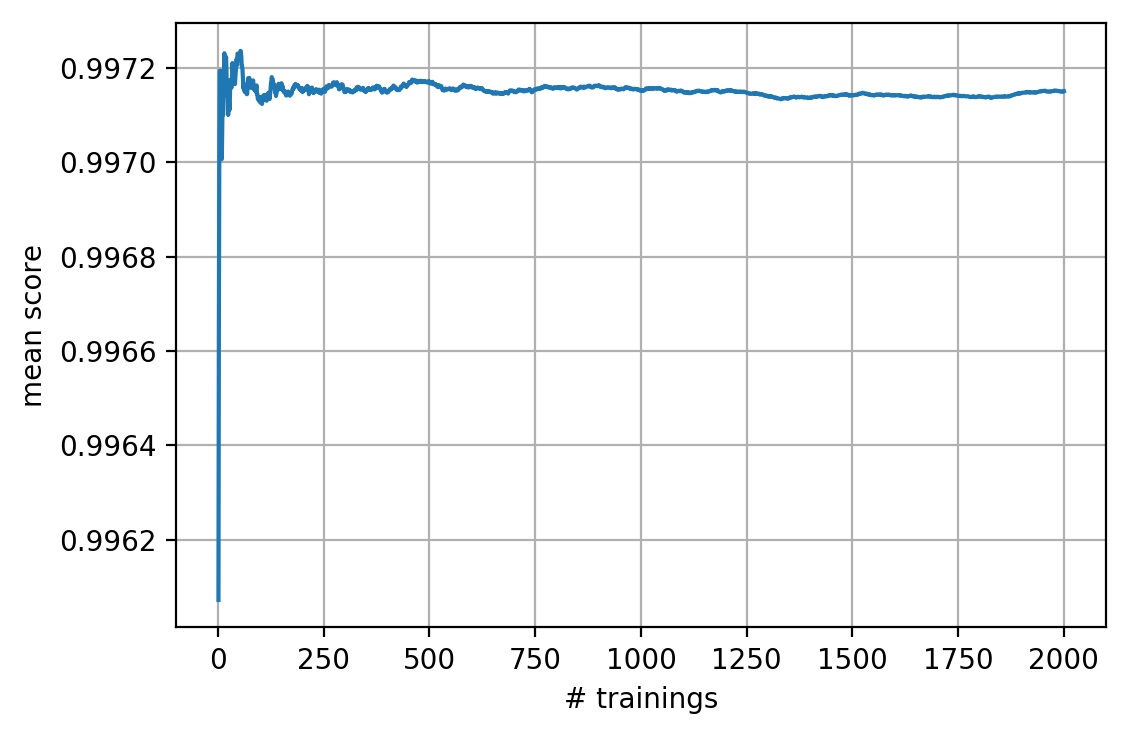
\includegraphics[width=0.32\textwidth]{./FigsClass/reg1_injmean_score}
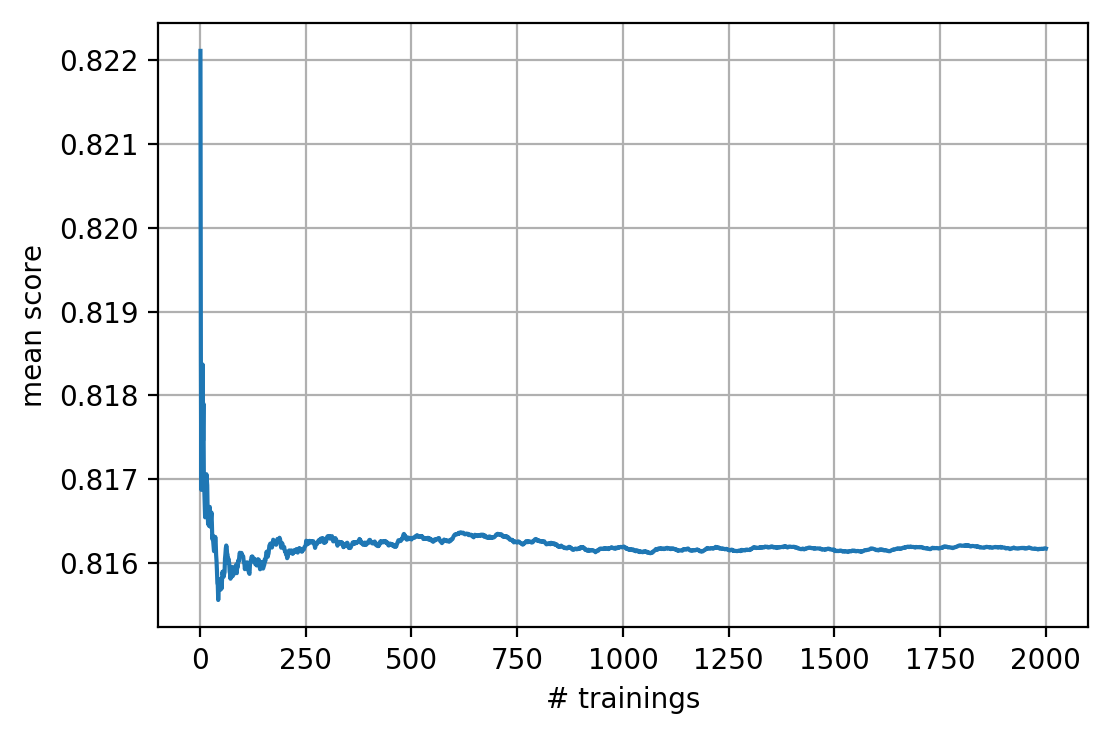
\includegraphics[width=0.32\textwidth]{./FigsClass/reg1_gstlalmean_score}
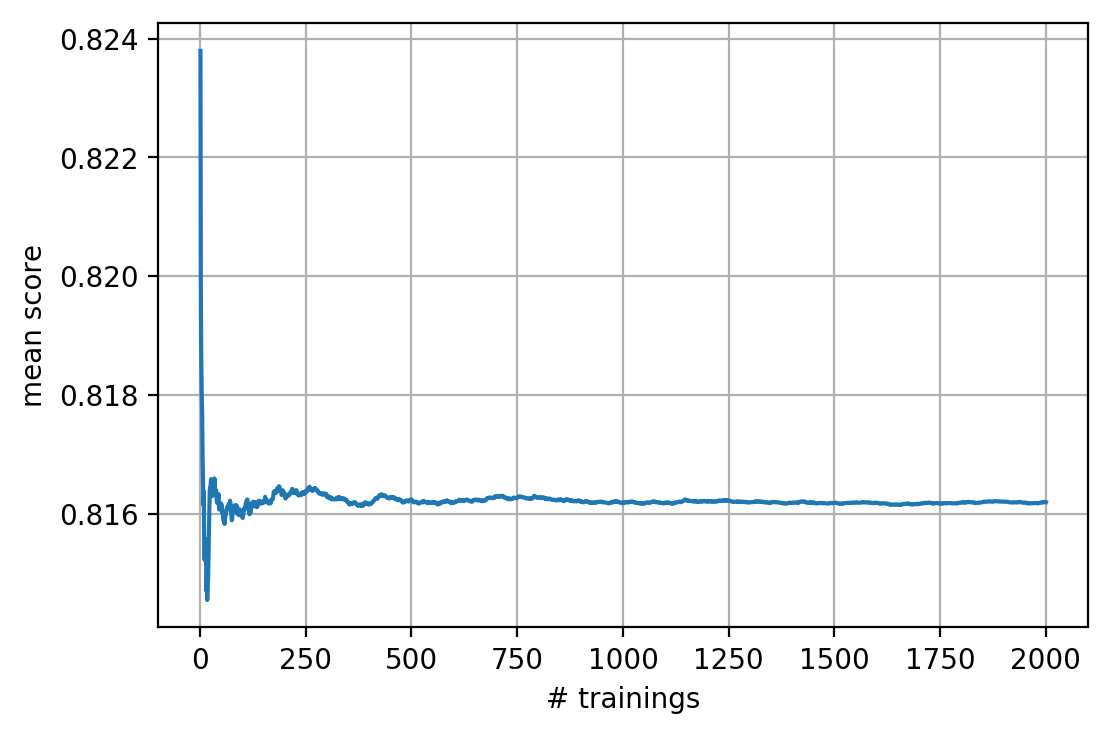
\includegraphics[width=0.32\textwidth]{./FigsClass/reg1_NNmean_score}
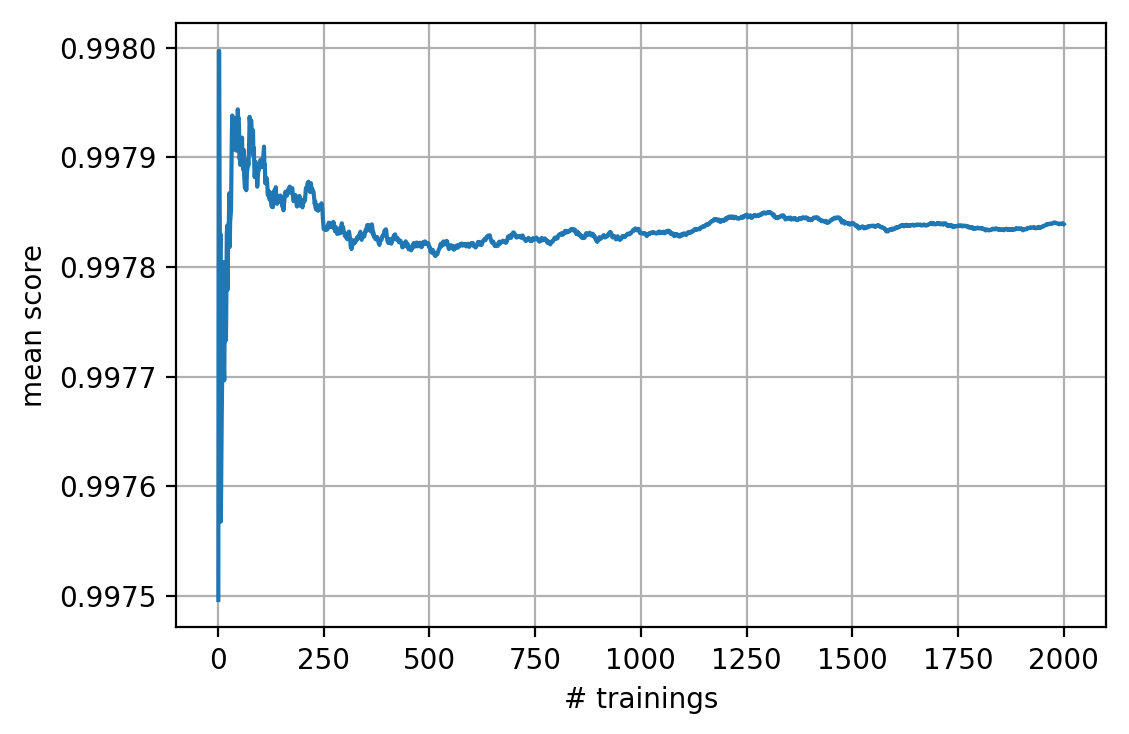
\includegraphics[width=0.32\textwidth]{./FigsClass/reg2_injmean_score}
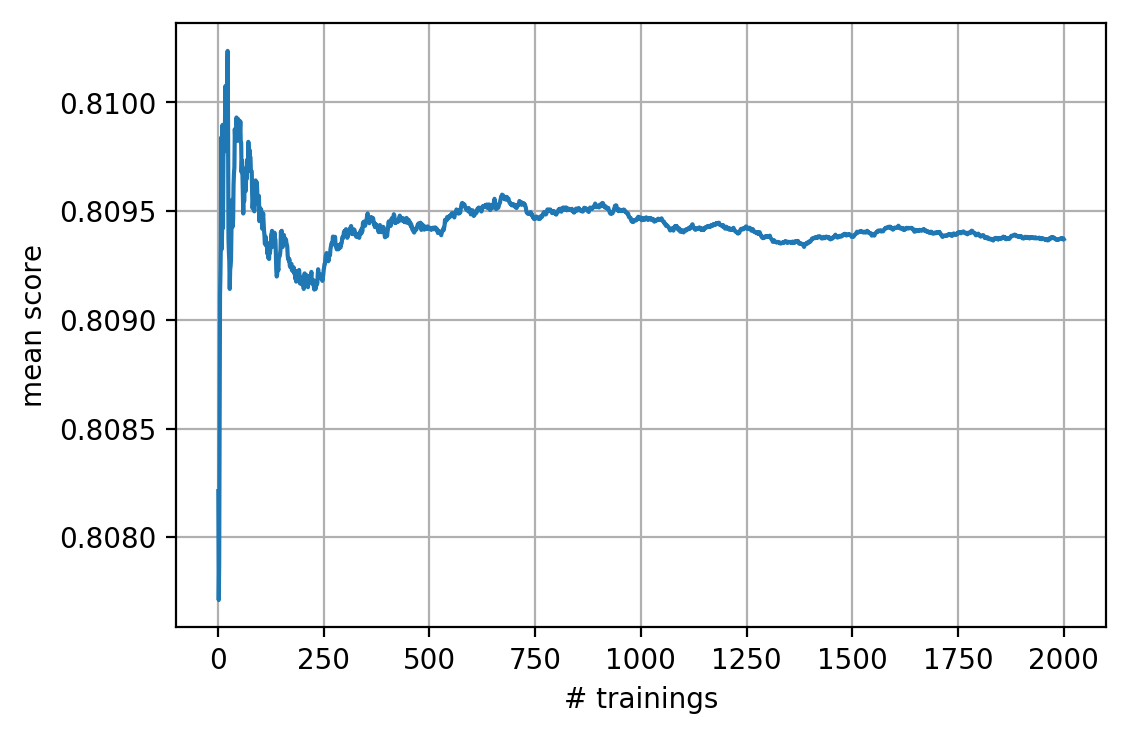
\includegraphics[width=0.32\textwidth]{./FigsClass/reg2_gstlalmean_score}
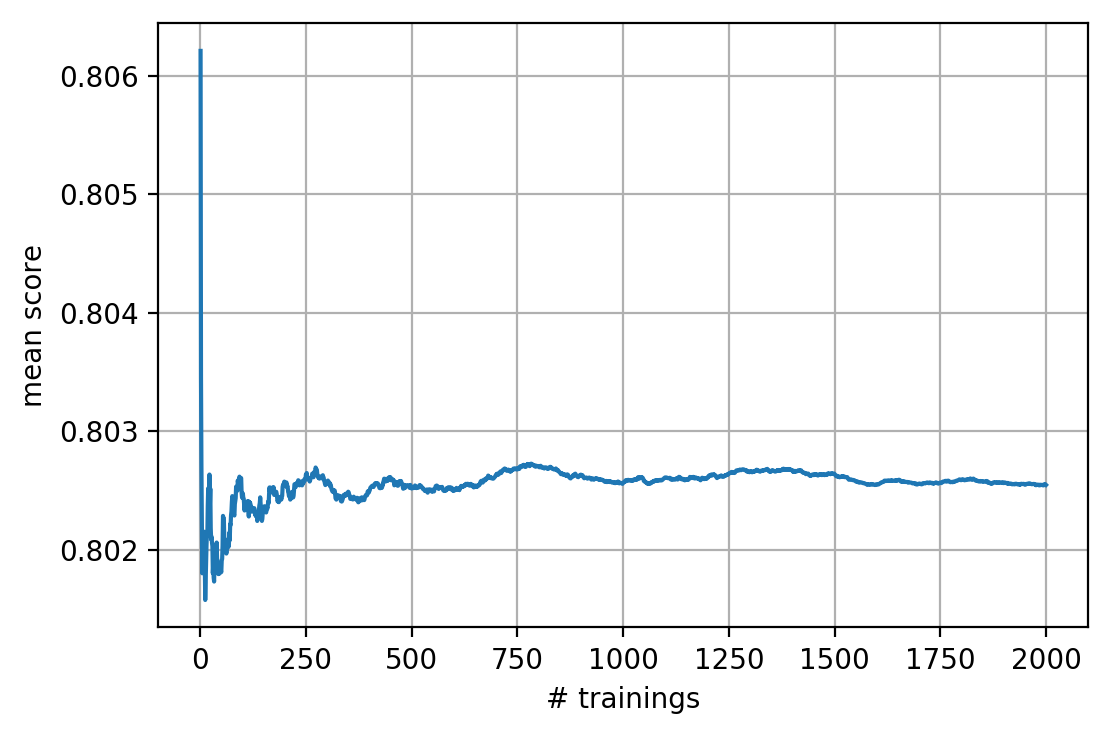
\includegraphics[width=0.32\textwidth]{./FigsClass/reg2_NNmean_score}
\caption{\label{fig:reg_mean} Evolution of the mean of the score with the number of trainings using injected data, recovered by gstlal and from the NN. Top three images are for \textbf{reg1}, and bottom three for \textbf{reg2}}
\end{figure*}

\begin{figure*}[]
\centering
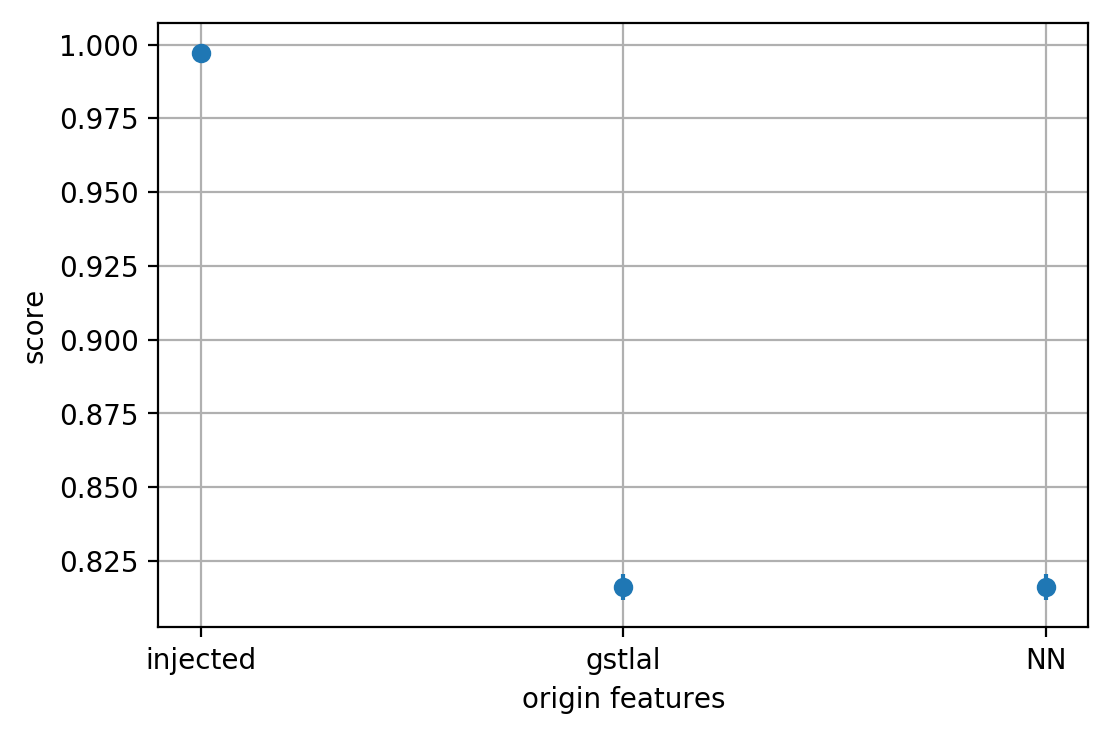
\includegraphics[width=0.45\textwidth]{./FigsClass/reg1_comparison}
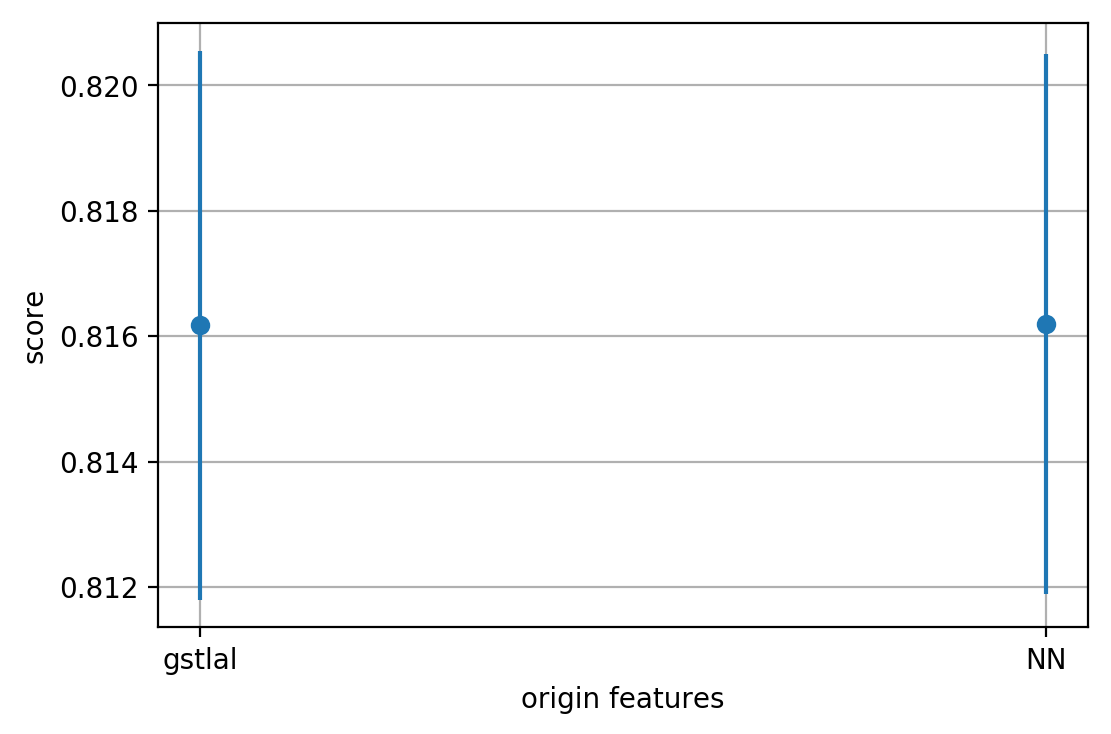
\includegraphics[width=0.45\textwidth]{./FigsClass/reg1_comparisonRecovered}
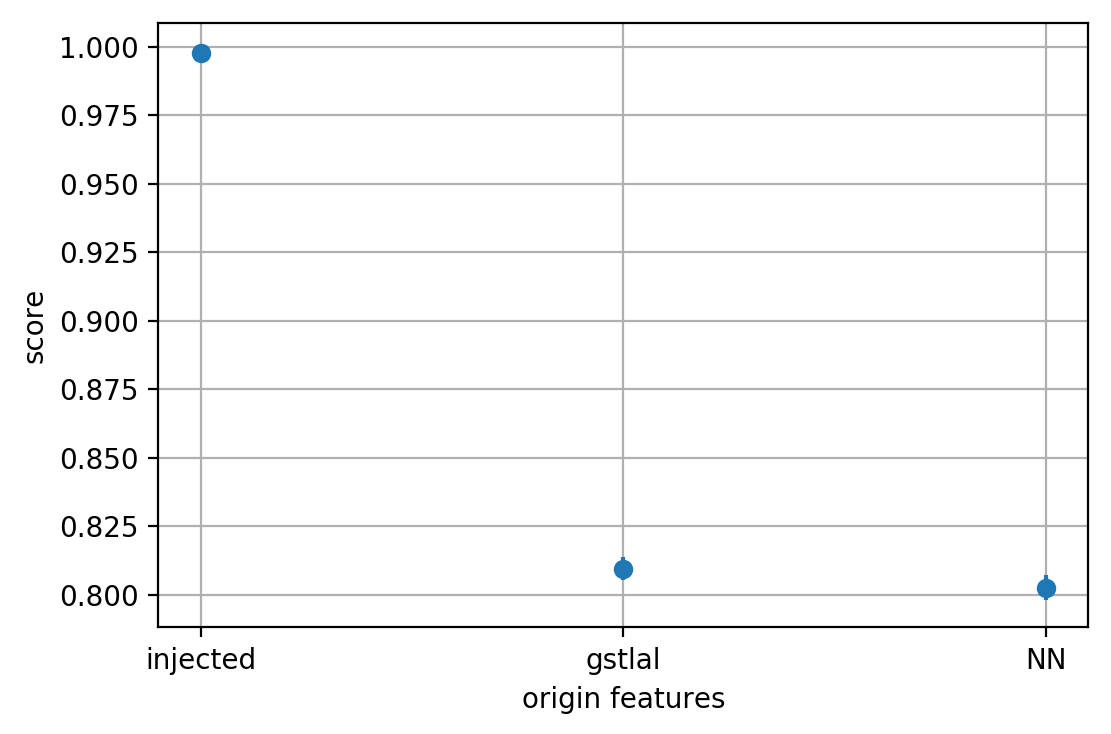
\includegraphics[width=0.45\textwidth]{./FigsClass/reg2_comparison}
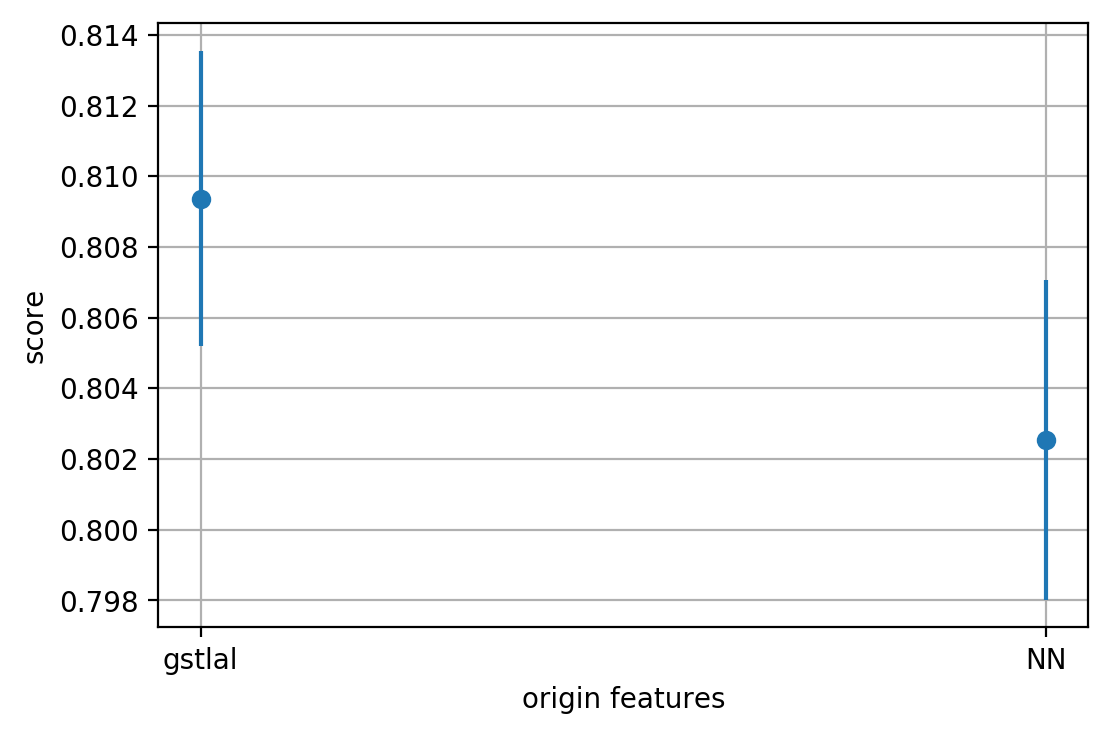
\includegraphics[width=0.45\textwidth]{./FigsClass/reg2_comparisonRecovered}
\caption{\label{fig:compareFirstTry} Comparison of the score between the three origins of the data. Top \textbf{reg1} and bottom \textbf{reg2}. On the left including the injected data, on the right just the recovered values.}
\end{figure*}


%==========================================================
\section{Fine tuning the parameters}
%==========================================================

Then we prepare a cross validation for some parameters that in previous studies showed important. 

We change the\textbf{ size of the forest} from 100 to 1000 trees. We expect the score to improve at some value in between, and then decrease again due to overfitting.

%Also we change the number of features used in each tree. As we only have two, we fix it as this number.

We also change the criterion for splitting between the two possible options: gini and entropy. Depending on the dataset, one usually give better results than the other.

As we know there is some dependency on the initial state and we do not want a bias in the cross validation, for every configuration we do 50 trainings and take as the score the mean. We also compute the standard deviation to compare the change with a configuration due to the initial state.

For \textbf{reg1} the results are in figure \ref{fig:cv_reg1}.

In the comparison of the mean score for different number of trees and information criterion, in every case the results are similar but differ. For gstlal, using the entropy criterion seems best in most cases, while criterion gini is best for data predicted from the NN. For the injected data one or another is preferred depending on the number of trees, but if we look at the score, the difference is in the fourth decimal place, so the configuration is not really relevant. It is not also very relevant in the other two, as we change just the third decimal position.

The maximum score is reached between 500 and 600 trees for the data that is not injected (there is pretty constant).

If we compare the two methods in the same plot, in the entropy criterion gstlal performs better than the NN. But in the plot with criterion gini, that was the best for the NN, also gstlal gets a better score in almost all cases. When using from 500 to 600 trees, the maximum score for both, then they are almost equal for gini, and gstlal is far better in entropy.

Conclusion: with cross validation we can get a slightly better score (changes in the third decimal position), but anyway the results are the same or better with the data extracted from gstlal than treated with the NN.

\begin{figure*}[]
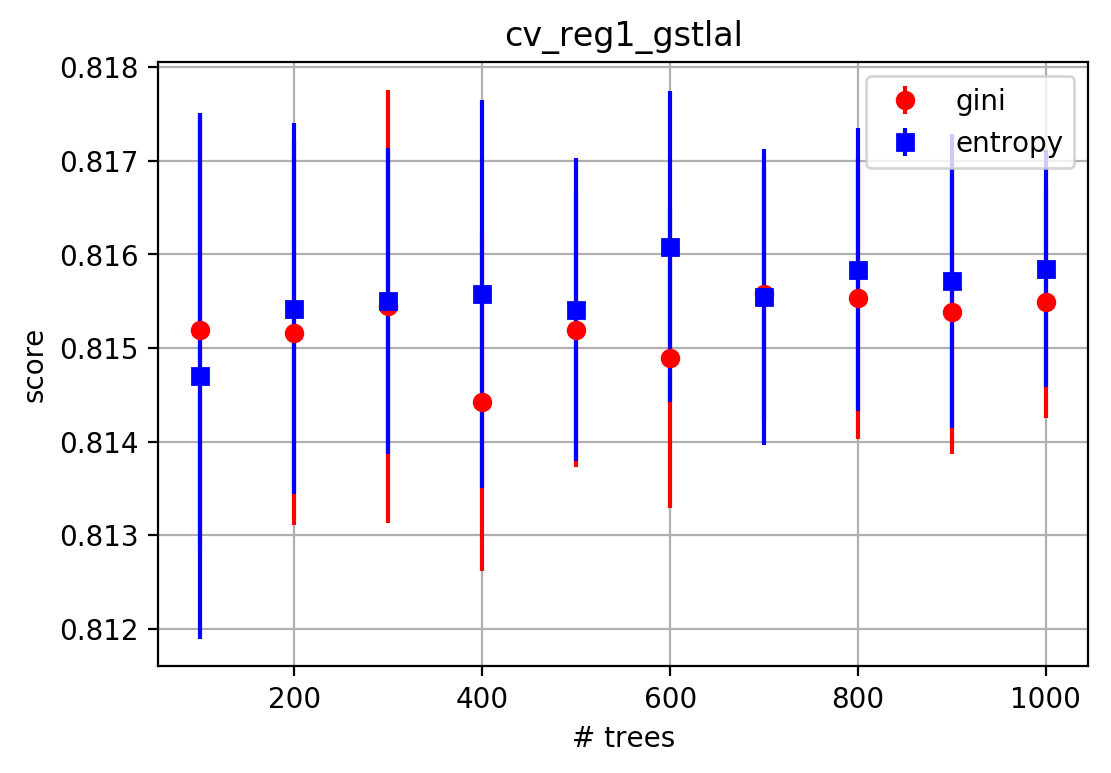
\includegraphics[width=0.32\textwidth]{./FigsClass/cv_reg1_gstlal}
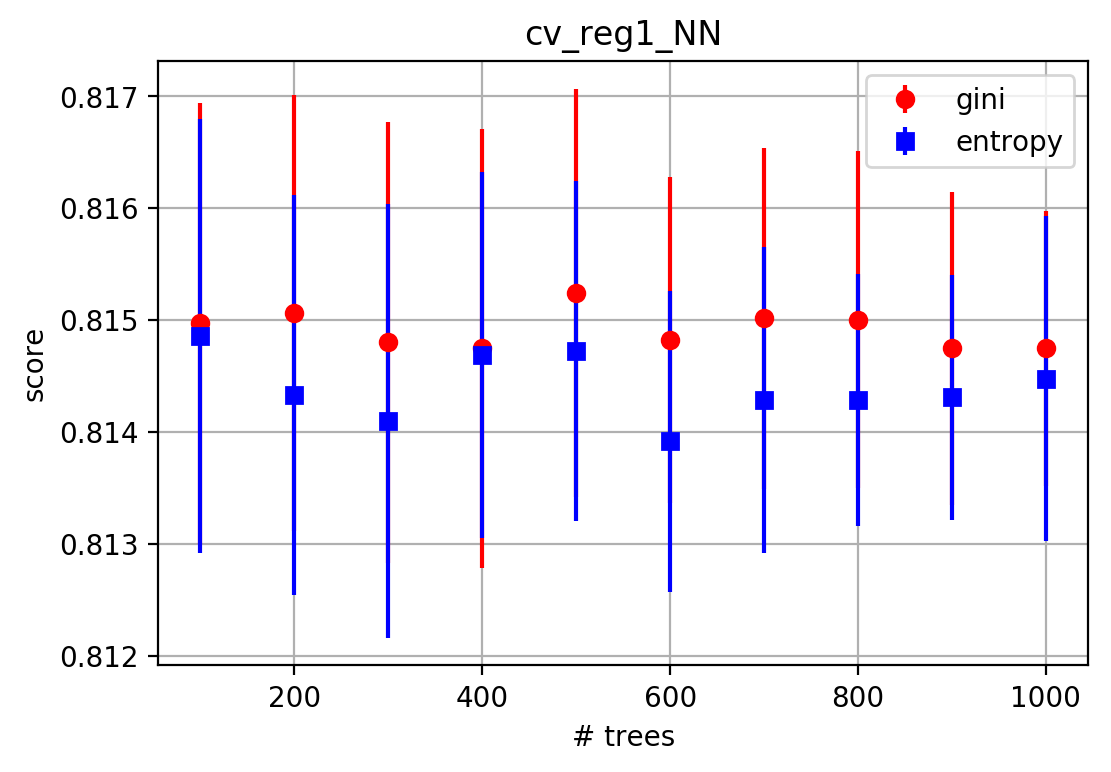
\includegraphics[width=0.32\textwidth]{./FigsClass/cv_reg1_NN}
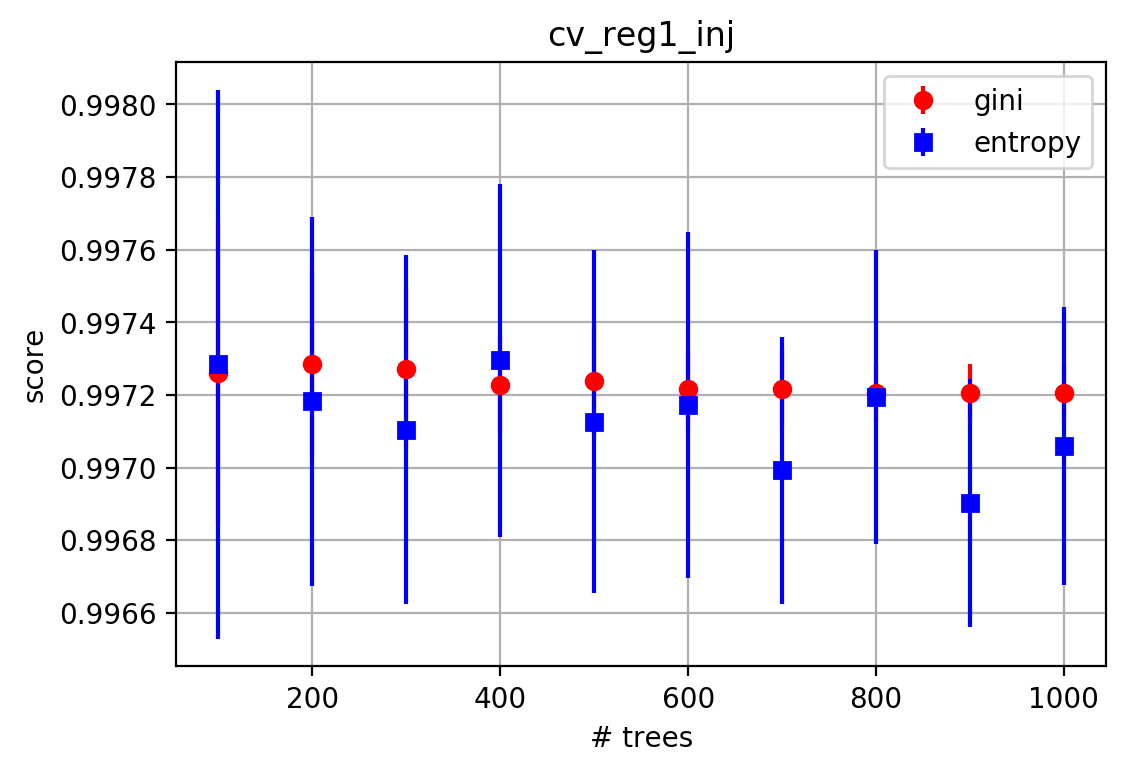
\includegraphics[width=0.32\textwidth]{./FigsClass/cv_reg1_inj}
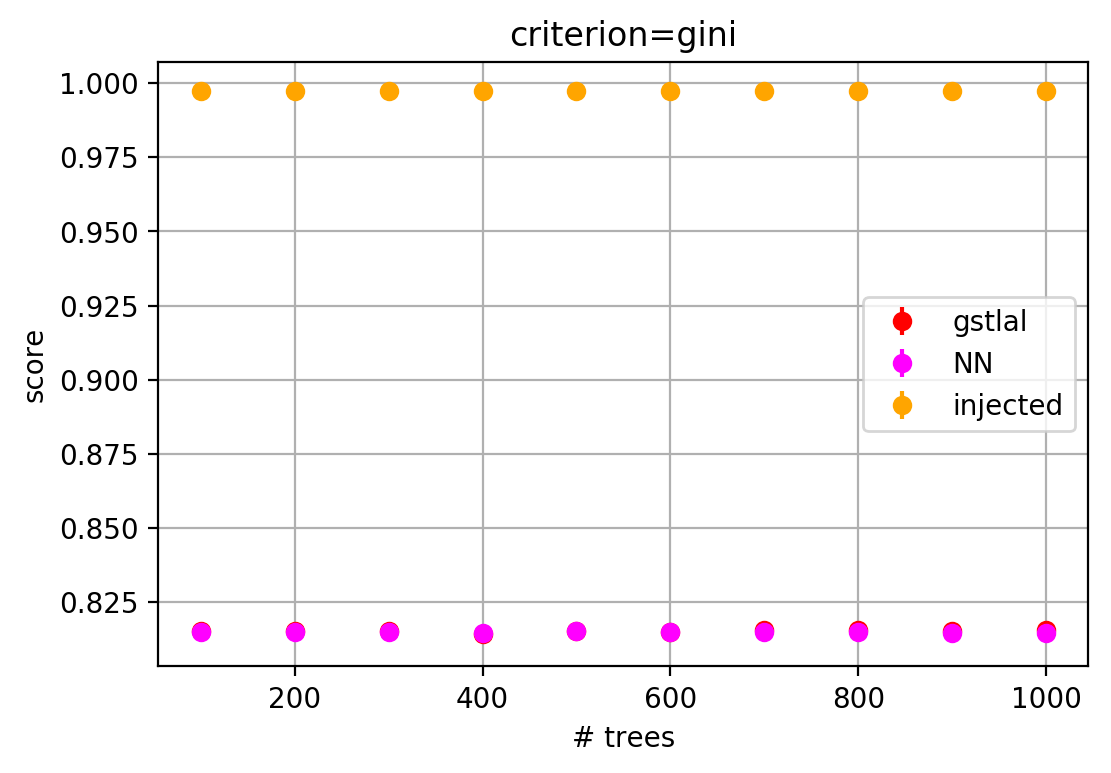
\includegraphics[width=0.45\textwidth]{./FigsClass/reg1_cv_comparisongini}
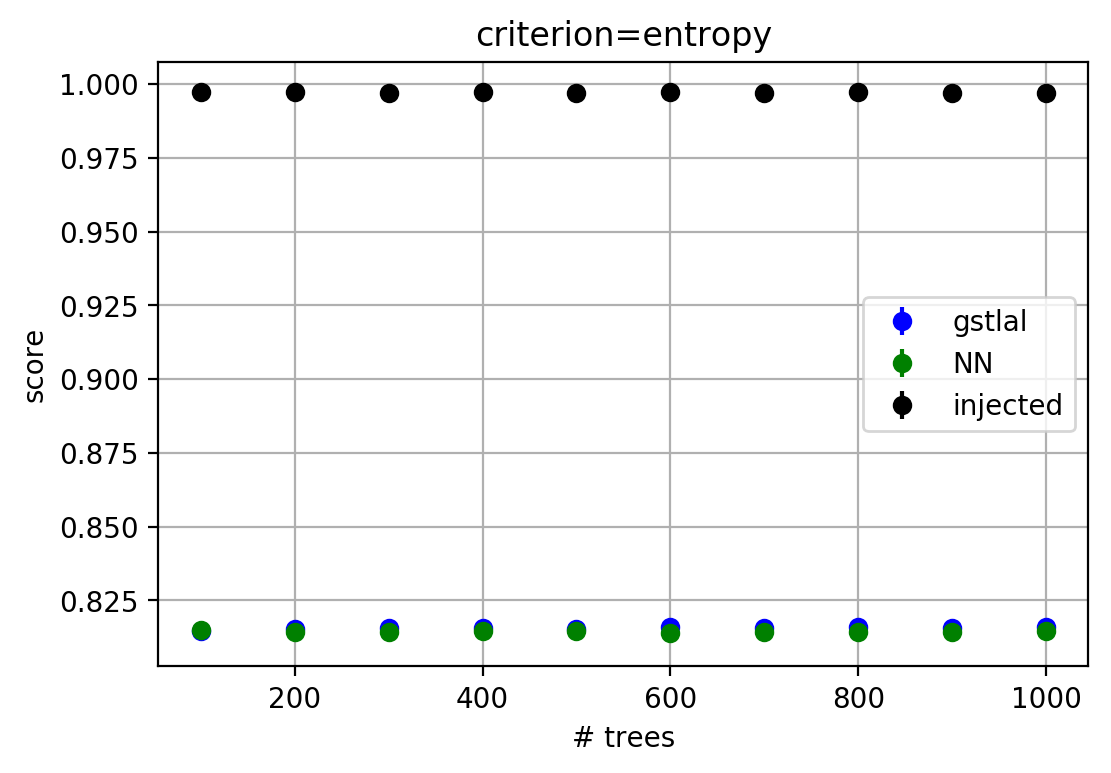
\includegraphics[width=0.45\textwidth]{./FigsClass/reg1_cv_comparisonent}
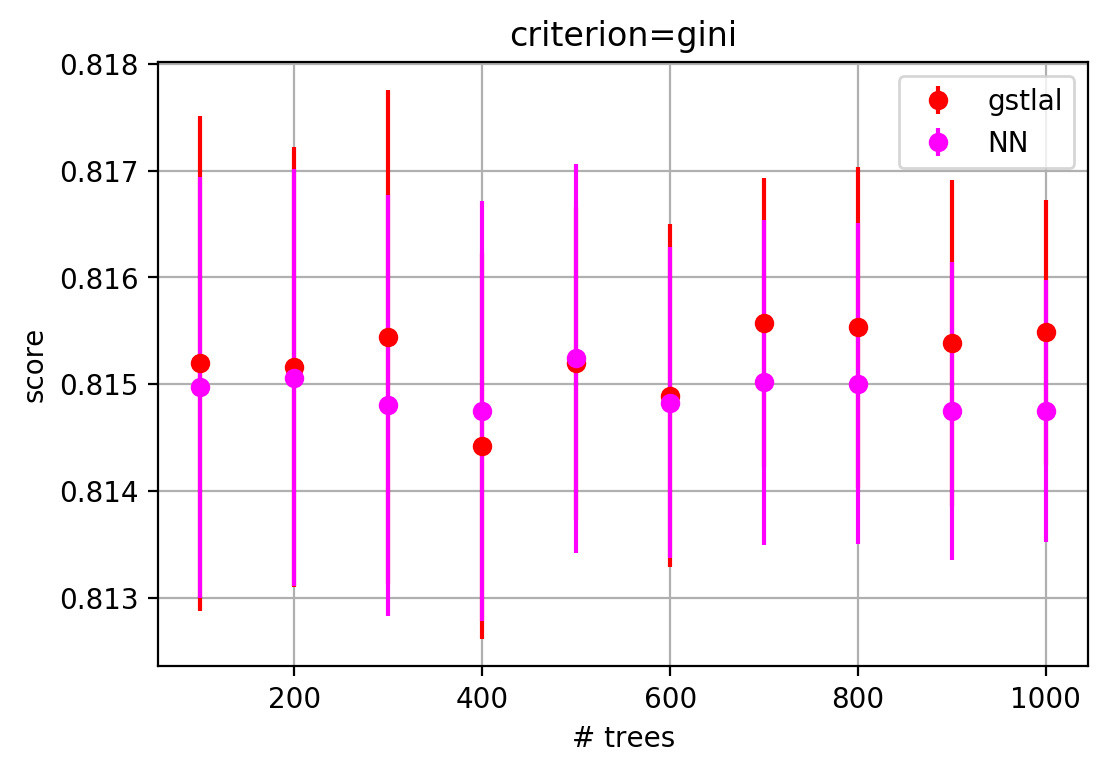
\includegraphics[width=0.45\textwidth]{./FigsClass/reg1_cv_2comparisongini}
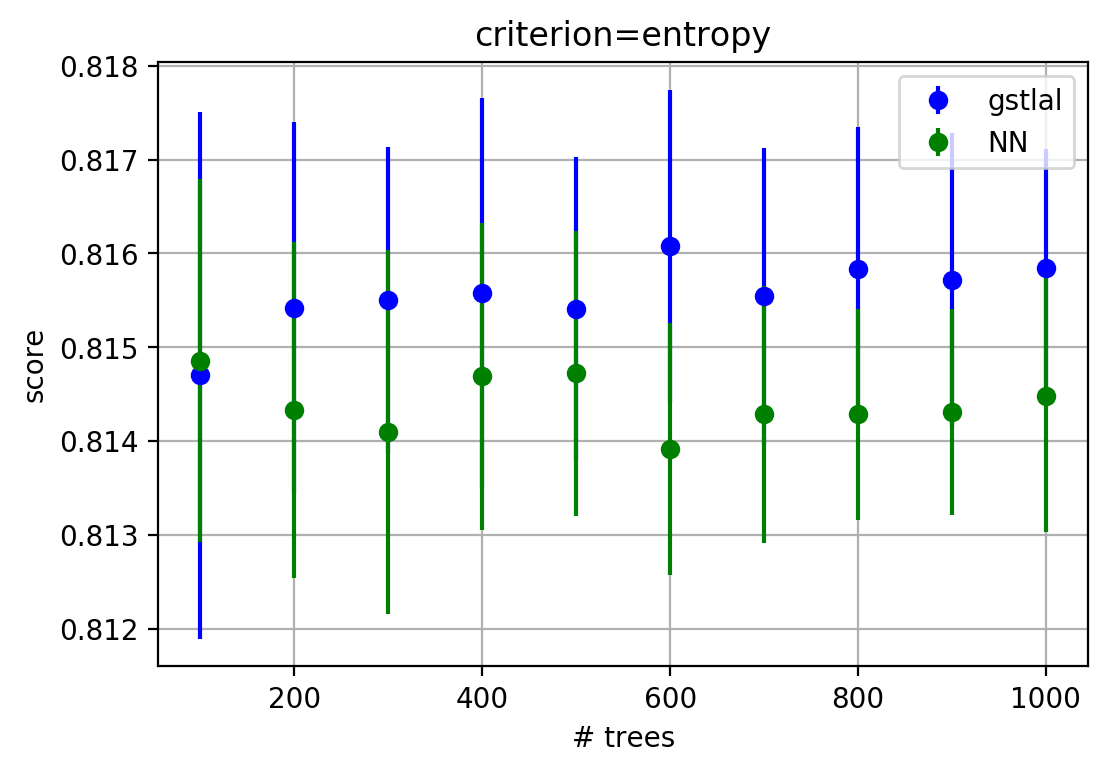
\includegraphics[width=0.45\textwidth]{./FigsClass/reg1_cv_2comparisonent}
\caption{\label{fig:cv_reg1} Cross validation on \textbf{reg1}. The top three plots show the score for different size of the forest and information criteria with the data from gstlal, predicted and injected. Then two plots show the comparison between the three of them. Finally we compare just gstlal vs predicted by NN}
\end{figure*}


%==========================================================
\bibliography{refs,local}
%==========================================================

\end{document}